\section{Цель выполнения лабораторной работы}
Целью выполнения лабораторной работы №1 является знакомство с специальными
электронными справочниками системного программиста и изучение принципов поиска
них информации по операционным системам, предназначенной для системного программиста.

\section{Порядок и условия проведения работы}
\begin{enumerate}
  \item Изучить в общем пособии (разделы 1,5,7) [6 – см. на сайте] разделы по: работе в режиме
        командной строки (КС) и по работе с файл-менеджерами (ФМ).
  \item В режиме КС запустить команды: DIR, HELP, DATE и SET. Продемонстрировать полученные
        навыки преподавателю ЛР.
  \item В программах FAR или VC (архив TASM3.ZIP – где 3 ЛР – на сайте) проверить: переключение
        каталогов, поиск файлов, создание и редактирование простого текстового файла, копирование
        и перемещение файлов, навигацию по меню. Продемонстрировать полученные навыки преподавателю ЛР.
  \item Скачать и развернуть справочники под эмулятором ОС (DOSBox v 7.4 – если на своем компьютере
        он не установлен, то скачать с сайта, установить, русифицировать и смонтировать виртуальный диск V:
        - см. ниже ) или в КС под CMD.EXE.
  \item Ответить устно на все контрольные вопросы ЛР.
  \item Изучить таблицу заданий для своего варианта
  \item Найти свою информацию по своему варианту и зафиксировать в отчете и изучить.
        СП 2024 год 2 курс ИУ5- 4-й сем. и 3-й курс ГУИМЦ 6-й семестр Большаков С.А.
  \item Изучить контрольные вопросы к ЛР и ответить на них.
  \item Показать ее преподавателю найденную информацию (демонстрация - отмечается в журнале)
  \item Оформить и распечатать отчет по своему варианту (шаблон в архиве этой ЛР).
  \item Защитить ЛР у преподавателя по контрольным вопросам (защита - отмечается в журнале
        и на титульном листе отчета).
\end{enumerate}

\section{Краткая инструкция по работе со справочником Help6}

\begin{enumerate}
  \item Справочник по варианту (Help 6) запускается через эмулятор DOSBox 0.74-3.
  \item Пропуск начальной заставки осуществляется нажатием любой клавиши:
  \item После появляется “Main Menu”:
        \begin{figure}[H]
          \begin{center}
            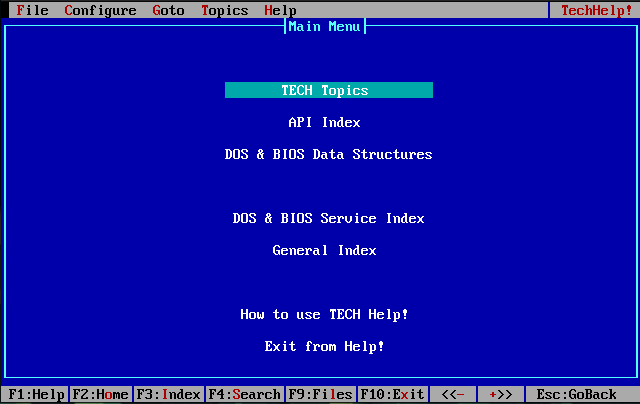
\includegraphics[scale=0.7]{3_help6_menu.png}
            \caption{Управление в справочнике Help6}
            \label{pic:pic_name}
          \end{center}
        \end{figure}
  \item В появившемся списке можно выбрать нужный раздел нажатием клавиши “Enter”:
        \begin{figure}[H]
          \begin{center}
            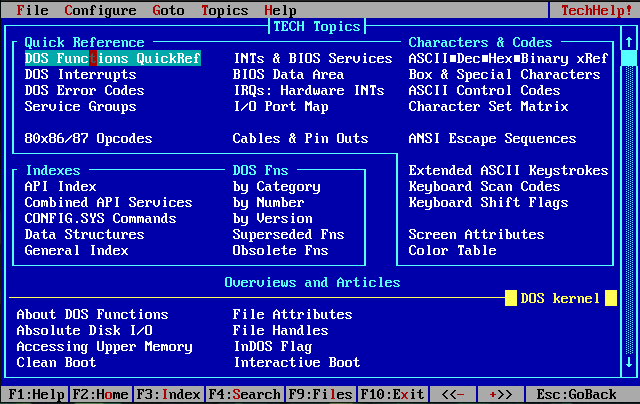
\includegraphics[scale=0.7]{3_help6_page.png}
            \caption{Управление в справочнике Help6}
            \label{pic:pic_name}
          \end{center}
        \end{figure}
  \item Аналогично для каждой темы и записи: по клавише “Enter” будет открываться подробное описание или содержание элемента.
  \item Для работы со справочником предусмотрены команды (посмотреть на F1):
        \begin{figure}[H]
          \begin{center}
            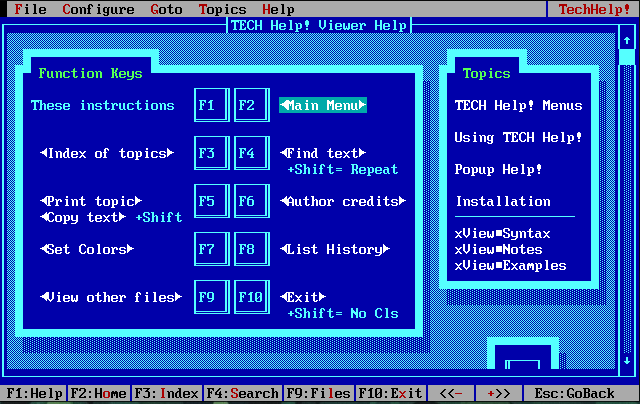
\includegraphics[scale=0.7]{3_help6_help}
            \caption{Управление в справочнике Help6}
            \label{pic:pic_name}
          \end{center}
        \end{figure}
\end{enumerate}

\section{Результаты поиска команды ОС}

Поиск команды произведем в справочнике Help5. Для этого обратимся в “DOS Commands”:

\begin{figure}[H]
  \begin{center}
    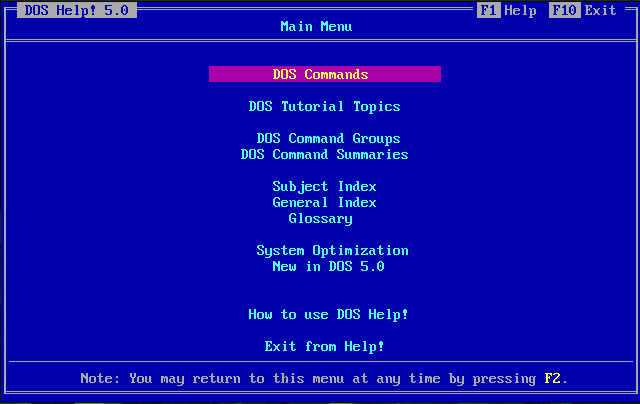
\includegraphics[scale=0.6]{4_help5_menu}
    \caption{}
    \label{pic:pic_name}
  \end{center}
\end{figure}

Найдем и выберем “Sort” и получим справку по блоку:

\begin{figure}[H]
  \begin{center}
    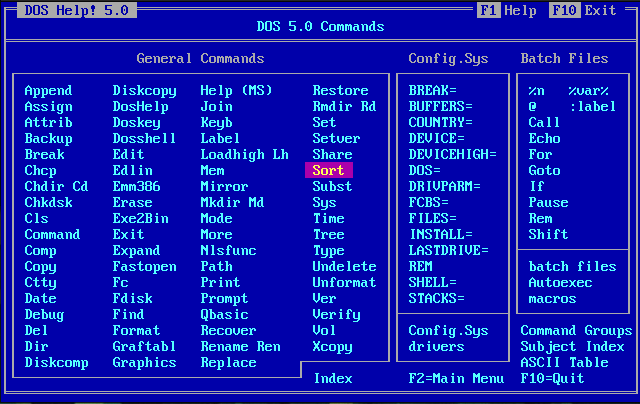
\includegraphics[scale=0.7]{4_help5_commands}
    \caption{}
    \label{pic:pic_name}
  \end{center}
\end{figure}

В данном разделе можно изучить команда Sort:

\begin{figure}[H]
  \begin{center}
    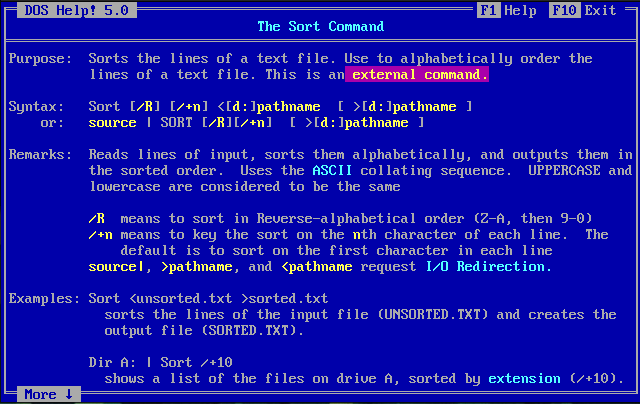
\includegraphics[scale=0.7]{4_sort_info_1}
    \caption{}
    \label{pic:pic_name}
  \end{center}
\end{figure}

\begin{figure}[H]
  \begin{center}
    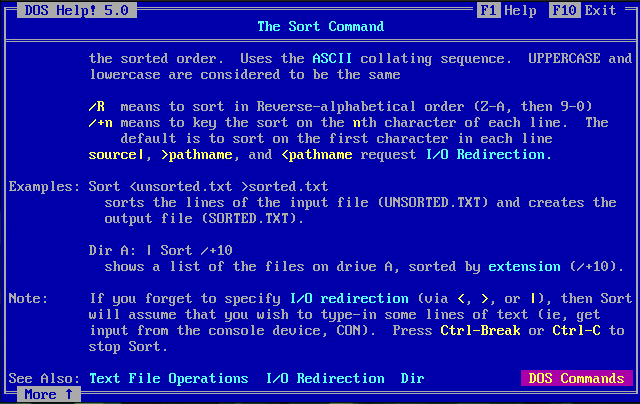
\includegraphics[scale=0.7]{4_sort_info_2}
    \caption{}
    \label{pic:pic_name}
  \end{center}
\end{figure}

Результат выполнения функции для .txt файла:

\begin{figure}[H]
  \begin{center}
    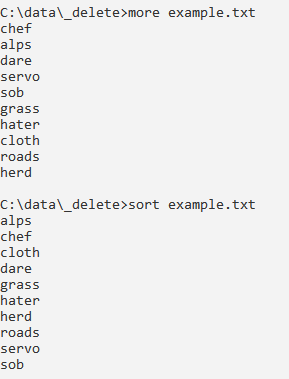
\includegraphics[scale=1]{4_sort_example}
    \caption{Пример использования команды Sort}
    \label{pic:pic_name}
  \end{center}
\end{figure}

\section{Результаты поиска прерывания ОС}

Поиск данного в варианте прерывания, переведенного в шестнадцатеричной системе счисления в 1eH, будет осуществляться в Help4.
\begin{figure}[H]
  \begin{center}
    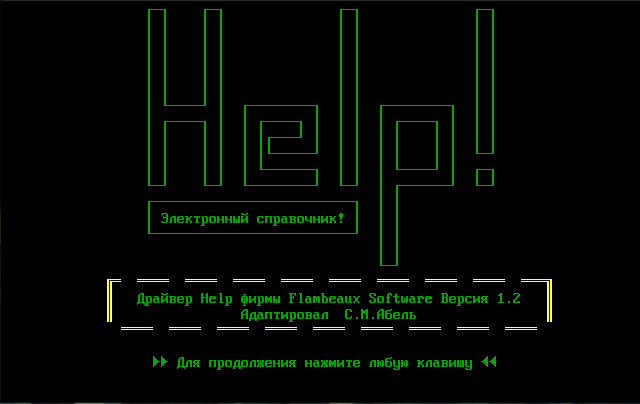
\includegraphics[scale=0.65]{5_help4_start.png}
    \caption{}
    \label{pic:pic_name}
  \end{center}
\end{figure}

Перейдем в разделы помощи:
\begin{figure}[H]
  \begin{center}
    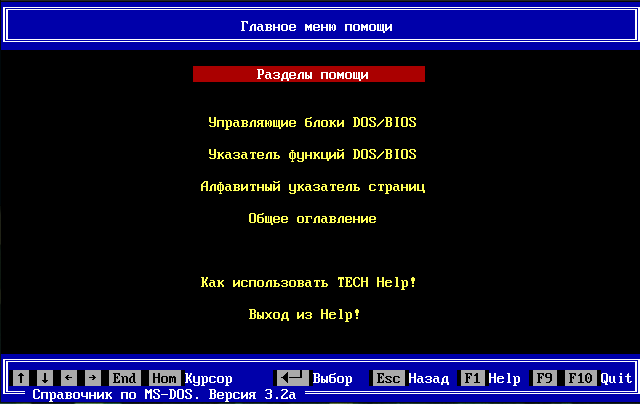
\includegraphics[scale=0.65]{5_help4_menu.png}
    \caption{}
    \label{pic:pic_name}
  \end{center}
\end{figure}

Затем в прерывания DOS:
\begin{figure}[H]
  \begin{center}
    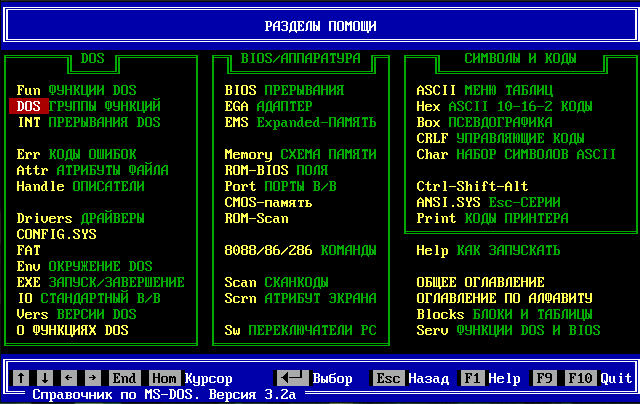
\includegraphics[scale=0.7]{5_help4_help.png}
    \caption{}
    \label{pic:pic_name}
  \end{center}
\end{figure}

Далее в символьный ввод-вывод:
\begin{figure}[H]
  \begin{center}
    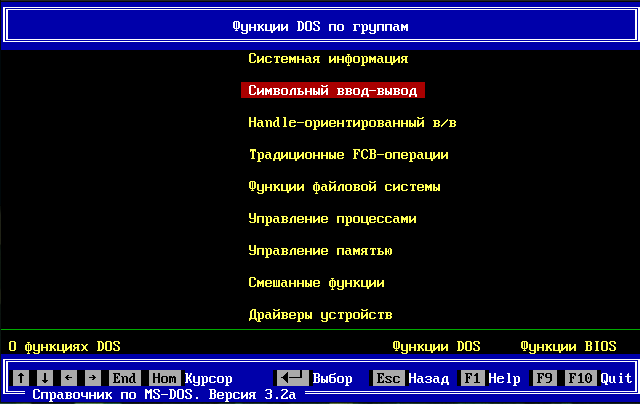
\includegraphics[scale=0.7]{5_help4_group.png}
    \caption{}
    \label{pic:pic_name}
  \end{center}
\end{figure}

Там выберем прерывание 09H, то есть 9 в шестнадцатеричной системе счисления:
\begin{figure}[H]
  \begin{center}
    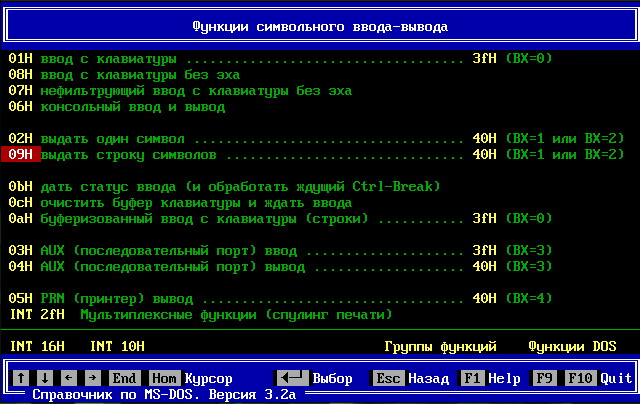
\includegraphics[scale=0.7]{5_help4_function.png}
    \caption{}
    \label{pic:pic_name}
  \end{center}
\end{figure}

И получим справку по необходимому нам прерыванию:
\begin{figure}[H]
  \begin{center}
    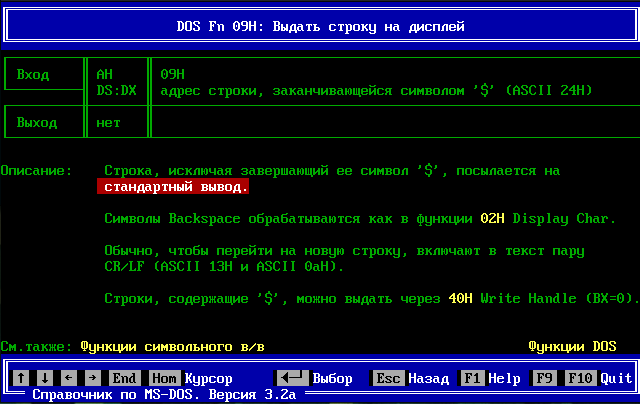
\includegraphics[scale=0.7]{5_help4_info.png}
    \caption{}
    \label{pic:pic_name}
  \end{center}
\end{figure}

\section{Результаты поиска управляющего блока ОС}

Описание структуры BPB можно найти в справочнике Help6.
Для этого выбираем раздел управляющие блоки DOS \& BIOS Data Structures:
\begin{figure}[H]
  \begin{center}
    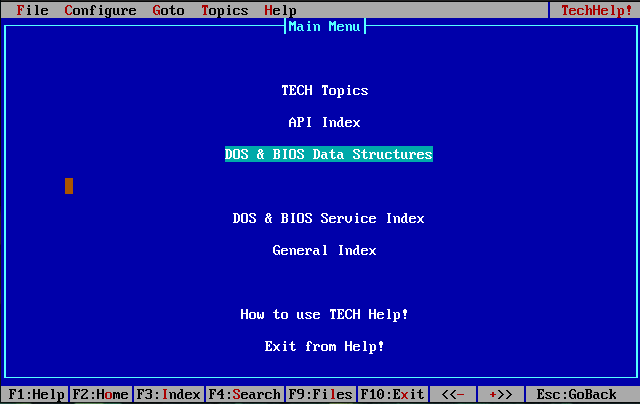
\includegraphics[scale=0.65]{6_help6_menu.png}
    \caption{}
    \label{pic:pic_name}
  \end{center}
\end{figure}

Выбираем блок MCB:
\begin{figure}[H]
  \begin{center}
    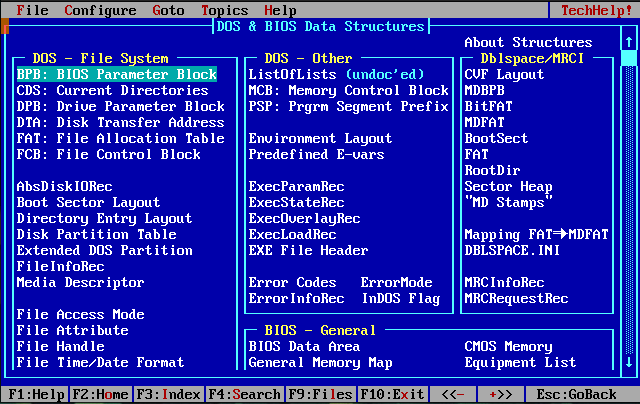
\includegraphics[scale=0.65]{6_help6_page.png}
    \caption{}
    \label{pic:pic_name}
  \end{center}
\end{figure}

И получаем справку по блоку:
\begin{figure}[H]
  \begin{center}
    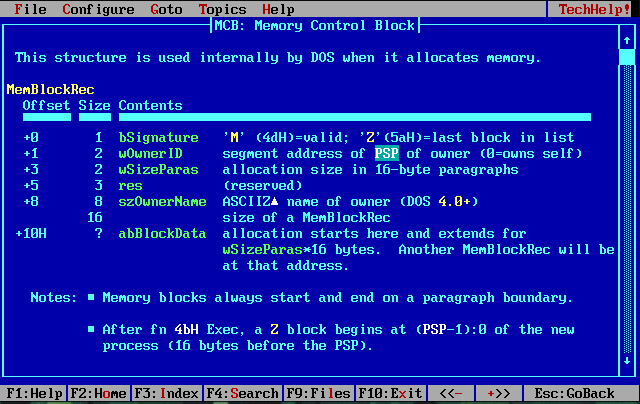
\includegraphics[scale=0.65]{6_mcb_1}
  \end{center}
  \begin{center}
    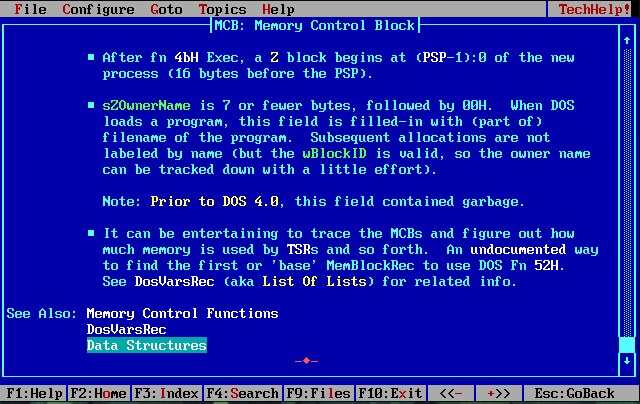
\includegraphics[scale=0.65]{6_mcb_2}
    \caption{MCB: Memory Control Block}
    \label{pic:pic_name}
  \end{center}
\end{figure}

\section{Выводы по ЛР}
В результате выполнения лабораторной работы была освоена работа с тремя справочниками,
получены навыки оперативного поиска информации о нужных командах, прерываниях и блоках
управления.
